

\begin{frame}
	~\\
	{\blank \textbf{RECAPS}
		\underline{Recap:}\\
		\begin{itemize}\blank
			\item Matrix-Vector Product:\\
			$A\in\mathbb{F}^{m\times n},~x\in\mathbb{F}^n$
			$$
			\begin{pmatrix}
			-&a_1&-\\~&\vdots&~\\-&a_m&-
			\end{pmatrix}
			\begin{pmatrix}
			x_1\\\vdots\\x_n
			\end{pmatrix}
			=\begin{pmatrix}
			(a_1,x)\\\vdots\\(a_m,x)
			\end{pmatrix}
			$$
			alternatively: $ Ax= x_1\begin{pmatrix}|\\a_1\\|\end{pmatrix}+\dots+x_n\begin{pmatrix}|\\a_n\\|\end{pmatrix} $
			\item Matrix-Matrix Product:\\
			$A\in\mathbb{F}^{m\times r},~B\in\mathbb{F}^{r\times n},~C\in\mathbb{F}^{m\times n}$\\
			illustrate dimensions for $A\cdot B=C$
			\item Image:\\
			Im$(A) :=\{Ax:~x\in\mathbb{F}^n\}$
			\item Kernel:\\
			ker$(A) := \{x\in\mathbb{F}^n:~Ax=0\}$
			\item Linear combination:
			$$
			\sum_{i=1}^{n} x_i\begin{pmatrix}|\\a_i\\|\end{pmatrix}
			=x_1\begin{pmatrix}|\\a_1\\|\end{pmatrix}+\dots+x_n\begin{pmatrix}|\\a_n\\|\end{pmatrix}
			$$
		\end{itemize}
	}
\end{frame}
\begin{frame}
		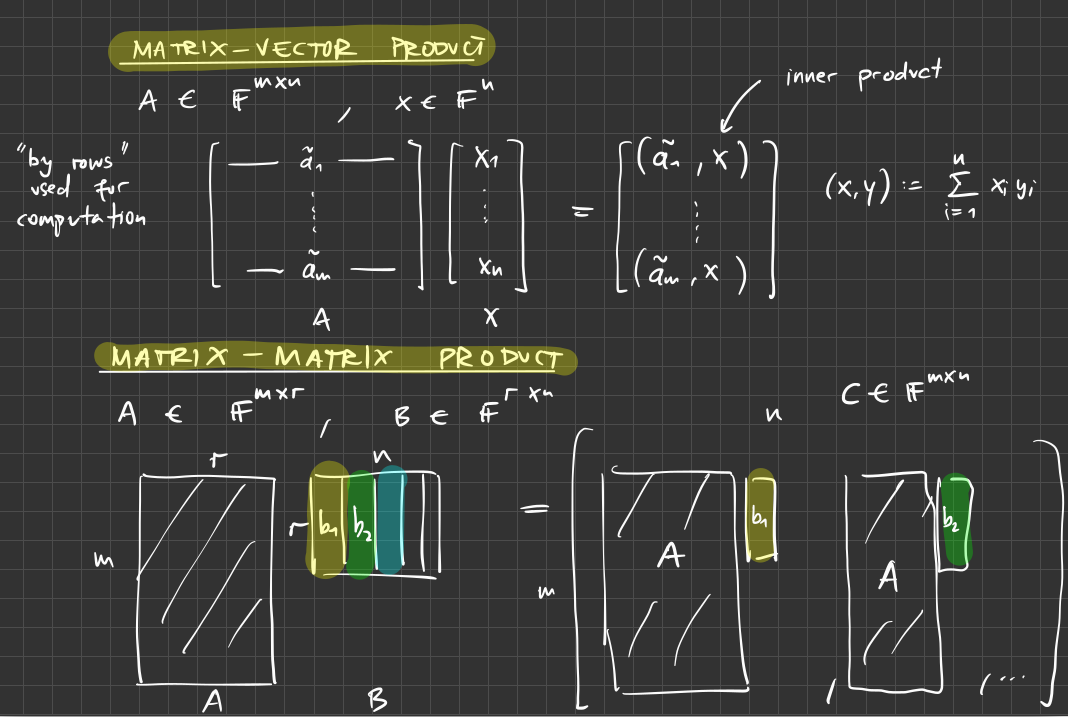
\includegraphics[width=0.99\linewidth]{../../rep/media/products}	
\end{frame}
\begin{frame}
	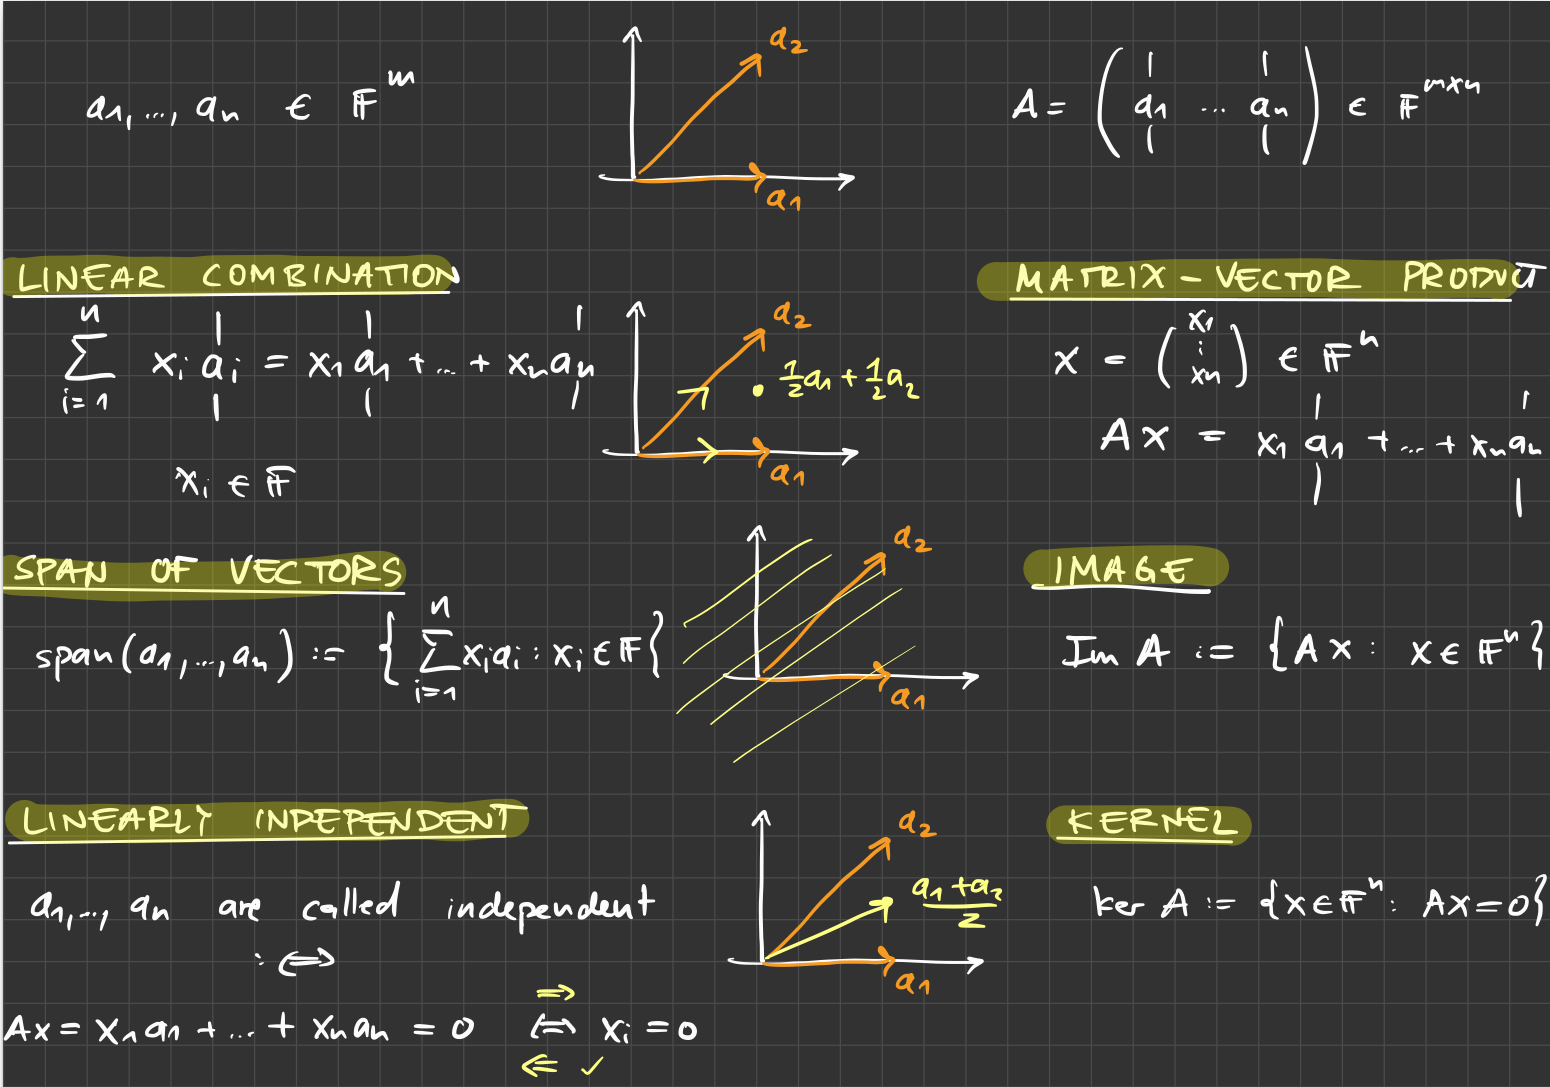
\includegraphics[width=0.99\linewidth]{../../rep/media/vectorVSmatrix.png}	
\end{frame}
\begin{frame}
	~\\
	{\blank
		\begin{itemize}\blank
			\item Span of vectors:
			$$
			\text{span}(a_1,\dots,a_n):=\lbrace \sum_{i=1}^{n}x_ia_i:~x_i\in\mathbb{F} \rbrace
			$$
			\item Linearly independent:
			\begin{align*}
			a_1,\dots,a_n~&\text{are called independent}\\
			&~~~~~~~~~:\Leftrightarrow\\
			Ax = x_1a_1&+\dots+x_na_n=0~~\Leftrightarrow~~x_i = 0
			\end{align*}
			\item Subspace of $\mathbb{F}^n$:\\
			$V\subset\mathbb{F}^n$ subspace $:\Leftrightarrow$\\
			$V\neq\emptyset$ and closed under linear combination $\lambda_1v_1+\lambda_2v_2\in V~~\forall~\lambda_1,\lambda_2\in\mathbb{F},v_1,v_2\in V$\\
			$\{v_1,\dots,v_r\}\subset V$ is called a basis of $V$, if
			\begin{itemize}\blank
				\item[i)]
				span$(v_1,\dots,v_r) = V~~~\Rightarrow~~\forall~v\in V~\exists_1\lambda\in\mathbb{F}^r:~v=\sum_{i=1}^{n}\lambda_iv_i$
				\item[ii)]
				$v_1,\dots,v_r$ linearly independent $\Rightarrow$ the scalars $\lambda_1,\dots,\lambda_r$ are uniquely defined
			\end{itemize}
			~\\
			One can show:\\
			Any basis of $V$ has the same length $r$, we set dim$(V)=:r$ (''dimension of $V$'')
		\end{itemize}
	}
\end{frame}
\begin{frame}
	~\\
	{\blank	
		\underline{Recap:}
		\begin{itemize}\blank
			\item \underline{Dimension formula:} $\forall~A\in\mathbb{F}^{m\times n}$:
			$$
			\underbrace{\text{dim}(\text{Im}(A))}_{\text{rank}(A)} + \underbrace{\text{dim}(\text{ker}(A))}_{\text{nullity}(A)} =\underbrace{n}_{\text{column dim.}}
			$$
			Let $m=n$:
			\item \underline{Inverse matrices:}
			$$
			A\in GL_n(\mathbb{F})~~:\Leftrightarrow~~\exists~A^{-1}\in\mathbb{F}^{n\times n}:~A^{-1}A=AA^{-1}=I
			$$
			\begin{itemize}\blank
				\item $A^{-1}$ is unique
				\item $\forall A,B\in GL_n(\mathbb{F}):~A\cdot B\in GL_n(\mathbb{F}),~(A\cdot B)^{-1}=B^{-1}\cdot A^{-1}$
				\item $\forall A\in GL_n(\mathbb{F}):~A^{-1}\in GL_n(\mathbb{F}),~(A^{-1})^{-1}=A$
				\item $D=\text{diag}(d_1,\dots,d_n)=\begin{pmatrix}d_1&~&0\\~&\ddots&~\\0& &d_n\end{pmatrix}~\text{invertible}~~\Leftrightarrow~~\forall i=1,\dots,n:~d_1\neq 0,~D^{-1}=\text{diag}(d_1^{-1},\dots,d_n^{-1})$
			\end{itemize}
		\end{itemize}
	}
\end{frame}

\begin{frame}
	~\\
	{\blank
		\underline{m=n:}
		\begin{align*}
		\begin{array}{rcl}
		\text{UNIQUENESS of solution}~\leftarrow~f_A~\text{injective}~\Leftrightarrow&ker(A)=\{0\}&\Leftrightarrow~a_1,\dots,a_n~\text{are linearly independent}\\
		~&\Updownarrow&~\\
		\text{EXISTENCE of solution}~\leftarrow~f_A~\text{surjective}~\Leftrightarrow&Im(A)=\mathbb{F}&\Leftrightarrow~\text{span}(a_1,\dots,a_n)=\mathbb{F}^n
		\end{array}
		\end{align*}
		$A=\begin{pmatrix}|&|\\a_1&a_2\\|&|\end{pmatrix}\in\mathbb{R}^{3\times 2},~~Ax=b$\\
		show image with vector outside the plane of $a_1,a_2$\\
		~\\
		$x,y\in\mathbb{R}^n:=\mathbb{R}^{n\times 1}$\\
		\begin{align*}
		(\bullet,\bullet)_2:~&\mathbb{R}^n\times\mathbb{R}^n\rightarrow\mathbb{R}\\
		&(x,y)_2=\sum_{i=1}^{n}x_iy_i
		\end{align*}
		$$ x^Ty=\begin{pmatrix}x_1&\cdots&x_n\end{pmatrix}\begin{pmatrix}y_1\\\vdots\\y_n\end{pmatrix}=(x,y)_2 $$
	}
\end{frame}
\begin{frame}
	~\\
	{\blank
		\underline{Recap:}\\
		\begin{itemize}\blank
			\item More Notation:\\
			Let $A=(a_{ij})_{ij}\in\mathbb{R}^{m\times n}$, then the transpose matrix $A^T=(a_{ij}')_{ij}\in\mathbb{R}^{n\times m}$ is defined by: $a_{ij}'=a_{ji}$
			\item Special case: Vectors
			$$
			\begin{pmatrix}|\\x\\|\end{pmatrix}\in\mathbb{R}^n:=\mathbb{R}^{n\times 1}~~
			\Rightarrow~~x^T=(x_1,\dots,x_n)\in\mathbb{R}^{1\times n}
			$$
			With this notation:
			$$
			(x,y)_2:=\sum_{i=1}^{n}x_iy_i =x^Ty = (x_1,\dots,x_n)\begin{pmatrix}y_1\\\vdots\\y_n\end{pmatrix}
			$$
			\item Notion of length: (norm)\\
			Für $x\in\mathbb{R}^n$ we define the Euclidean norm by
			$$
			\|\bullet\|_2:~\mathbb{R}^n\rightarrow[0,+\infty),~x\mapsto \|x\|_2:=\sqrt{x^Tx}=\sqrt{\sum_{i=1}^{n}x_i^2}
			$$
			\item Cauchy-Schwarz Inequality:
			$$
			\forall~x,y\in\mathbb{R}^n:~|x^Ty|\leq\|x\|_2\cdot\|y\|_2
			$$
			We find: $\forall~x,y\in\mathbb{R}^n\setminus\{0\}~~\exists_1~\alpha\in (0,\pi):~\text{cos}(\alpha)=\frac{x^Ty}{\|x\|_2\cdot\|y\|_2}$
		\end{itemize}
	}
\end{frame}

\begin{frame}
	~\\
	{\blank
		\begin{itemize}\blank
			\item Projections:
			\begin{align*}
			\frac{x^Ty}{\|x\|\cdot\|y\|}&=~\text{cos}(\alpha) = \frac{l}{\|y\|}~~\Leftrightarrow~~l=\frac{x^Ty}{\|x\|}\\
			\text{proj}_x(y)&=l\cdot\frac{x}{\|x\|}=\frac{x^Ty}{\|x\|}\cdot\frac{x}{\|x\|}\\
			\|\text{proj}_x(y)\|&=\|l\cdot\frac{x}{\|x\|}\|\\
			&=l\cdot\|\frac{x}{\|x\|}\|\\
			&=l\cdot\frac{1}{\|x\|}\cdot \|x\|=l
			\end{align*}
			\item Orthogonal matrices and vectors:
			\begin{align*}
			x,y~\text{orthogonal}~~&\Leftrightarrow~~\text{cos}(\alpha)=0~~\Leftrightarrow~~x^Ty\\
			Q=\begin{pmatrix}
			|&~&|\\q_1&\cdots&q_n\\|&~&|
			\end{pmatrix}\in\mathbb{R}^{n\times n}~\text{orthogonal}~~&\Leftrightarrow~~Q^TQ = I\\
			&\Leftrightarrow~~q_1,\dots,q_n~\text{are mutually orthonormal}
			\end{align*}
		\end{itemize}¸
	}
\end{frame}

\begin{frame}
	~\\
	{\blank
		\begin{itemize}\blank
			\item QR-Decomposition and Gram-Schmidt Algorithm:\\
			$\forall~A\in\mathbb{R}^{m\times n} (m\geq n),~\exists Q\in\mathbb{R}^{m\times m}~\text{orthogonal},~R\in\mathbb{R}^{m\times n}~\text{upper triangular}:~A=Q\cdot R$
			\begin{align*}
			a_1 &= r_{11}q_1\\
			a_2 &=r_{12}q_1+r_{22}q_2
			\end{align*}
			\underline{IDEA:}\\
			draw $a_i,q_i,\tilde{q}_i$ for $A=\begin{pmatrix}2&1\\0&2\end{pmatrix}$
			\begin{align*}
			&\tilde{q}_1:=a_1,\\
			&q_1:= \frac{\tilde{q}_1}{\|\tilde{q}_1\|}=\frac{1}{\|a_1\|}a_1=\frac{1}{2}\begin{pmatrix}2\\0\end{pmatrix}\\
			&\tilde{q}_2:=a_2-\frac{a_1^Ta_2}{\|a_1\|}q_1\\
			&q_2:=\frac{\tilde{q}_2}{\|\tilde{q}_2\|}
			\end{align*}
		\end{itemize}
	}
\end{frame}

\begin{frame}
	~\\
	{\blank
		\underline{Recap:}
		\begin{align*}
		\text{DETERMINANT}&=~\text{number that we assign to a square matrix}~A\in\mathbb{F}^{n\times n}\\
		&=~\text{''measure for linear independence''}\\
		\end{align*}
		illustrate $|\text{det}(A)|=2$-dim. volume for $A=\begin{pmatrix}|&|\\a_1&a_2\\|&|\end{pmatrix}$\\
		~\\
		\underline{Crucial:}\\
		-Important result:
		$$
		A\in GL_n(\mathbb{F})~~\Leftrightarrow~~\text{det}(A)\neq 0
		$$\\
		-Laplace formula:
		$$
		\text{det}(A)~=~\sum_{j=1}^{n} (-1)^{i+j} a_{ij} ~\text{det}(A_{ij})
		$$
	}
\end{frame}